\documentclass[12pt,a4paper,twoside]{scrartcl}
\usepackage{fancyhdr} %für Kopf- und Fußzeilen
\usepackage[utf8x]{inputenc} %Zeichenkodierung
\usepackage[english]{babel} %Sprache (ngerman für Deutsch)
\usepackage{graphicx} %für Bilder
\usepackage[printonlyused, withpage]{acronym} %für die Abkürzungsliste
\usepackage{caption}
\usepackage{calc}
\usepackage{hhline}
\usepackage{multirow} 
\usepackage{xcolor}
\usepackage{colortbl}
\usepackage{booktabs}
\usepackage{setspace}
\usepackage{listings}
\usepackage{color}
\usepackage{enumitem} %Anpassbare Enumerates/Itemizes
\usepackage{tikz}
\usepackage{relsize}
\usepackage{pdfpages}
\usepackage{placeins}
% \usepackage{subfig}
\usepackage{xspace}
\usepackage{mathtools}
% \usepackage[demo]{graphicx}
\usepackage{subcaption}

%Kreiert Links von der Table of Content zu Kapiteln (ohne optische Hervorhebung)
\usepackage[pdftex,pdfborder={0 0 0},plainpages=false]{hyperref}
\usepackage[left=2.5cm,right=2.5cm,top=2.5cm,bottom=3cm,includeheadfoot]{geometry}
\usepackage{url}
\usepackage{float}

%set check and cross mark
\newcommand{\cmark}{\ding{51}}
\newcommand{\xmark}{\ding{55}}

\newcommand{\para}[1]{\noindent{\textbf{#1}}}

\newcommand{\TODO}[1]{\textcolor{red}{TODO: #1}}
\newcommand{\TODOP}[1]{\textcolor{red}{TODO: #1}}
\newcommand{\TODOX}[1]{\textcolor{red}{TODO: #1}}
\newcommand{\NOTE}[1]{\textcolor{blue}{\textbf{NOTE}: #1}}
\newcommand{\DONEX}[1]{\textcolor{blue}{#1}}
\newcommand{\catI}{Sampling Algorithms\xspace}
\newcommand{\catII}{Filtering Algorithms\xspace}
\newcommand{\catIII}{Data Sharing\xspace}


%import time.sty for time charts
\usetikzlibrary{arrows}

%set XML language
\definecolor{darkblue}{rgb}{0.0,0.0,0.6}
\lstdefinelanguage{XML}
{
  morestring=[b]",
  morestring=[s]{>}{<},
  morecomment=[s]{<?}{?>},
  stringstyle=\color{black},
  identifierstyle=\color{darkblue},
  keywordstyle=\color{cyan},
  morekeywords={xmlns,version,type}% list your attributes here
}

% Set title color
\definecolor{titlecolor}{RGB}{0,0,0}
%\titleformat*{\section}{\normalfont\Large\bfseries\color{titlecolor}}
%\titleformat*{\subsection}{\normalfont\large\bfseries\color{titlecolor}}
%\titleformat*{\subsubsection}{\normalfont\normalsize\bfseries\color{titlecolor}}

\clubpenalty = 10000 % verhindert "Schusterjungen" (Einzelzeile unten)
\widowpenalty = 10000 \displaywidowpenalty = 10000 % verhindert "Hurenkinder" (Einzelzeile oben)
 
\newcommand{\student}{Alexander Dadiani}	%Hier Name eintragen
\newcommand{\kurs}{}					%Hier Kurs eintragen
\newcommand{\lokation}{Berlin}		%Hier „Heimat“-Lokation eintragen
\newcommand{\matrikel}{365739}		%Hier Matrikelnummer eintragen
\newcommand{\vondatum}{DD/MM/YYYY}	%Hier Startdatum eintragen (mm/dd/yyyy)
\newcommand{\bisdatum}{DD/MM/YYYY}	%Hier Enddatum eintragen (mm/dd/yyyy)
\newcommand{\berichttitel}
	{A catalogue of sampling algorithms for sensor data}
% \newcommand{\berichtuntertitel}
	% {Here comes the subtitle}
\newcommand{\sture}{Prof. Dr. Volker Markl / Prof. Dr. Rüdiger Zarnekow}%Hier Supervisor1 eintragen
\newcommand{\betreuer}{Traub, Jonas}%Hier Supervisor2 eintragen
\newcommand{\abgabedatum}{02/28/2019}		%Hier Abgabedatum eintragen (mm/dd/yyyy)

%Add environment to mark draft sections
\newcommand{\draftcontent}[2]{
	{\leavevmode\color{red}\textbf{Notice: The following content, marked grey, is just a scratch/preview.}}	
	{\leavevmode\color{red}\textit{#1 \newline}}
	{\leavevmode\color{black!50}#2}	
}
\newcommand{\nocontent}[1]{
	{\leavevmode\color{red}\textbf{Notice: Unfortunately, this part of the thesis not available yet.}}	
	{\leavevmode\color{red}\textit{#1 \newline}}
}

%set italic text for acronyms
\renewcommand*{\acsfont}[1]{\textit{#1}}
\renewcommand*{\acffont}[1]{\textit{#1}}
\renewcommand*{\acfsfont}[1]{\textit{#1}}

%Reconfigure autoref
\let\subsectionautorefname\sectionautorefname
\let\subsubsectionautorefname\sectionautorefname

\hypersetup{ 
  pdftitle={Bachelor Thesis - \berichttitel - \student}, %%
  pdfauthor={\student}, %%
%   pdfsubject={\berichtuntertitel}, %%
}

%%%%

\title{\berichttitel}
\author{\student}
\date{\abgabedatum}

\newlength{\iconwidth}
\setlength{\iconwidth}{1cm}

\definecolor{boxheadcol}{gray}{.6}
\definecolor{boxcol}{gray}{.9}

\begin{document}

%%%%%%%%%%% title page
\begin{titlepage}
 \begin{center}
  \includegraphics*[height=3cm]{images/Logos/TUBerlin_Logo.png}
  \linebreak
  {\Large\textbf {Technische Universität Berlin}}\\
   \vspace{3.5cm}

  {\Large\textbf{Bachelor Thesis}}\\
  \vspace{0.7cm}  
  {\begin{onehalfspace}\Huge\textbf \textsf{\berichttitel} \end{onehalfspace}}
  \vspace{0.5cm}
%   \berichtuntertitel\\
  %{\large \vondatum\ -- \bisdatum}\\
  \vspace{2.5cm}
  {\textbf \student}\\
  \vspace{0.1cm}
  \kurs
  \vspace{0.1cm}
  Matriculation \#: \matrikel\\
  \vspace{0.3cm}
  \textbf{Supervisors:} \sture \\
  \textbf{Advisors:} \betreuer \\  
  \vspace{0.5cm}
  \abgabedatum
 \end{center}
\end{titlepage}
\clearpage
\mbox{}
\thispagestyle{empty}
\clearpage

%%%%%%%%%%%%%%%%%%%%%%%%%%%%%%%%%%%%%%%%%%%%%%%%%%
%externes Deckplatt
%\includepdf{images/Titelblatt.pdf}
%\thispagestyle{empty}   
%\cleardoublepage
%%%%%%%%%%%%%%%%%%%%%%%%%%%%%%%%%%%%%%%%%%%%%%%%%%

\pagestyle{fancy}
\lhead{}
\chead{\rightmark}
\rhead{}

\cfoot{\small \student: \berichttitel}
\lfoot{\ifthispageodd{}{\thepage}}
\rfoot{\ifthispageodd{\thepage}{}}
%\rfoot{\thepage}

\fancyhfoffset{\marginparsep}
\renewcommand{\footrulewidth}{1.0pt}
\renewcommand{\headrulewidth}{1.0pt}
\renewcommand{\headheight}{30pt}
\pagenumbering{roman}

%%Listing
%\lstset{
%	tabsize=2,
%	language=Java,
%	basicstyle=\small,
%	keywordstyle=\color{blue!80!black!100},
%	identifierstyle=,
%	showstringspaces=false,
%	commentstyle=\color{green!50!black!100},
%	stringstyle=\ttfamily,
%	breaklines=true,
%	numbers=left,
%	numberstyle=\tiny,
%	numbersep=5pt,
%	frame=single,
%	backgroundcolor=\color{white},
%	aboveskip=0.2cm,
%	captionpos=b
%}

% Default settings for code listings
 \lstset{frame=tb,
   aboveskip=3mm,
   belowskip=3mm,
   showstringspaces=false,
   columns=flexible,
   basicstyle={\footnotesize\ttfamily},
   numbers=left,
   numberstyle=\tiny\color{gray},
   keywordstyle=\color{blue},
   commentstyle=\color{green!50!black!100},
   stringstyle=\color{purple},
   frame=single,
   breaklines=false,
   breakatwhitespace=false,
   tabsize=2,
   language=java,
   captionpos=b,
   frame=bt
 }

\onehalfspacing
\parindent 0pt
\parskip 12pt

%%%%%%%%%%% Declaration of Academic Honesty
% May replace this with the declaration of your institution...
\thispagestyle{empty}

\section*{Erklärung (Declaration of Academic Honesty)}

Hiermit erkläre ich, dass ich die vorliegende Arbeit selbstständig und
eigenhändig sowie ohne unerlaubte fremde Hilfe und ausschließlich unter
Verwendung der aufgeführten Quellen und Hilfsmittel angefertigt habe.  

\textit{I hereby declare to have written this thesis on my own and without forbidden help of others, using only the listed resources.}

\vspace{2cm}
\begin{tabular}{p{5cm} p{4cm} p{5cm}}\cline{1-1}\cline{3-3}
Datum &  & \student
\end{tabular}

\clearpage
\thispagestyle{empty}   
\cleardoublepage

%%%%%%%%%%%% inner title page
%\includepdf{images/XXX.pdf}
%\thispagestyle{empty}   
%\cleardoublepage

%%%%%%%%%%% table of contents
\setcounter{page}{3}
\begin{spacing}{0.0}
\tableofcontents
\end{spacing}
\clearpage

%%%%%%%%%%% list of figures, listings and tables

\clearpage
\singlespacing
\addcontentsline{toc}{section}{List of Figures}
\listoffigures
\clearpage
\addcontentsline{toc}{section}{List of Listings}
\renewcommand{\lstlistlistingname}{List of Listings}
\lstlistoflistings
\addcontentsline{toc}{section}{List of Tables}
\listoftables
\clearpage

%%%%%%%%%%% acronyms
\section*{List of Acronyms}
\addcontentsline{toc}{section}{Acronyms}
\begin{acronym}[YTM]
\acro{RSN}   {Rechargeable Sensor Network}
\acro{WSN}   {Wireless Sensor Network}
\acro{SN}    {Sensor Network}
\acro{CS}    {Compressive Sampling}
\acro{MSE}   {Mean Squared Error}
\acro{SI}    {Sampling Interval}
\acro{SIR}   {Sampling Interval Range}
\acro{CI}    {Confidence Interval}
\acro{USAC}  {Utility-based Sensing and Communications Protocol}
\acro{PEWMA} {Probabilistic Exponential Weighted Moving Average}
\acro{EWMA}  {Exponential Weighted Moving Average}
\acro{EASA}  {Energy Aware Adaptive Sampling Algorithm}
\acro{ASA}   {adaptive Sampling Algorithm}
\acro{FFT}   {fast Fourier Transform}
\acro{CDG}   {compressive Data Gathering}
\acro{DCT}   {Discrete cosine transform}
\acro{STCDG} {Spatio-Temporal Compressive Data Collection}
\acro{EDCA}  {Efficient Data Collection Approach}
\acro{SVD}   {Singular value decomposition}
\acro{NMAE}  {Normalized Mean Absolute Error}
\acro{SQL}   {Structured Query Language}
\acro{MVN}   {Multivariate Normal Distribution}
\end{acronym}
\clearpage
\mbox{}
\thispagestyle{empty}
\clearpage

%%%%%%%%%%% content
\pagenumbering{arabic}
\interlinepenalty 1000
%!TEX root = jt-thesis-main.tex

\section{English Abstract}
\begin{onehalfspace}
	
	The english abstract is required for all english theses at TU-Berlin.
\end{onehalfspace}
\clearpage

\section{Deutscher Abstract}
\begin{onehalfspace}
	
	Ein deutscher Abstract wird immer benötigt, für alle Abschlussarbeiten an der TU-Berlin. 
\end{onehalfspace}
\clearpage

\section{Introduction}
\label{sec:Introduction}
% cite: ~\cite{hirzel2014catalog}
% footnote \footnote{footnotes working fine}
Gartner Inc. states that the number of interconnected devices will reach 20.4 billion by 2020 \footnote{Gartner Inc., R. (2017, February 7). Gartner Says 8.4 Billion Connected "Things" Will Be in Use in 2017, Up 31 Percent From 2016. Retrieved September 28, 2018, from https://www.gartner.com/en/newsroom/press-releases/2017-02-07-gartner-says-8-billion-connected-things-will-be-in-use-in-2017-up-31-percent-from-2016}.
To gather information from those devices, we need algorithms which efficiently sample and route data from sensor nodes (i.e., devices) to data sinks. Energy expenditure will gain higher importance, especially for mobile devices such as battery-powered wearables and smartphones. Wireless Sensor Networks (WSNs) are often battery-powered and use cases span from home and health applications to the military sector~\cite{akyildiz2002wireless}. With low production costs of a node as a goal in WSNs~\cite{akyildiz2002wireless}, resource usage at the nodes is restricted. While reducing sampling frequencies leads to a higher life of a battery-powered sensor network, important changes in the observed phenomenon could be missed which reduces the quality of the data~\cite{akyildiz2002wireless}. A tradeoff between the quality of data and energy expenditure arises, thus an optimization is needed. Different methods for optimizing WSNs were presented in surveys (e.g.,~\cite{abbasi2007survey},~\cite{sivrikaya2004time},~\cite{carrano2014survey}). The proposed areas of optimization include clustering algorithms~\cite{abbasi2007survey}, time synchronization~\cite{sivrikaya2004time}, duty cycling~\cite{carrano2014survey}, topology control~\cite{li2013survey}, in-network aggregation~\cite{fasolo2007network}, data compression~\cite{srisooksai2012practical}, and general routing techniques~\cite{al2004routing}~\cite{kulkarni2011particle}~\cite{singh2015survey}~\cite{rault2014energy}. TinyDB~\cite{madden2005tinydb}, ACQUIRE~\cite{sadagopan2003acquire} and COUGAR~\cite{yao2002cougar} introduce system architectures for query processing which consist of algorithms for sampling, and routing data requested by a user through a SQL-like language.




\subsection{Motivation}
\label{sec:motivation}

As stated above, surveys and taxonomies were presented for different areas of sensor networks. However, during our research, we did not encounter a survey or catalog focusing on sampling algorithms in sensor networks. This thesis aims to provide a catalog for a comprehensive overview of the existing sampling algorithms for the specific use case of sensor data. For researchers as well as practitioners, a collection of sampling algorithms is a valuable starting point for finding a solution for a design problem in a sensor network. Thus, a taxonomy of the algorithms will be presented to provide a compact overview. Furthermore, algorithms which focus on areas other than sensing (like routing and topology building) in sensor networks will be presented. Combinations of said algorithms with sampling algorithms as well as combinations of sampling algorithms from different categories could inspire further research.

\subsubsection{Scientific Background}
\label{sec:Scientific Background}

Different types of sensor networks, like wireless, rechargeable, or wired sensors networks exist. 
However, some algorithms are designed for a specific type of network. For example, AdaM~\cite{trihinas2015adam} can be applied to all kinds of networks, while the algorithm presented by Santini and Romer~\cite{santini2006adaptive} is designed for wireless sensor networks. Other algorithms build upon existing architectures, for example, TiNA~\cite{sharaf2003tina} expands the TinyDB framework with a temporal coherency tolerance to prevent the transmission of slight data changes. Some sampling and filtering algorithms implemented in SNs were initially designed for special use cases and architectures. For example, an algorithm by Alippi et al.~\cite{alippi2010adaptive} was initially designed for a snow monitoring application, however, the authors argue that it is usable in other cases where the monitored phenomenon is slowly changing over time, too. Other algorithms are more general and suited for a range of applications and use cases (e.g.,~\cite{fan2013fast}~\cite{gaura2013edge})


\clearpage
\subsection{Contributions}
\label{sec:contributions}

Clearly point out and describe the contributions of this work

The contributions of this thesis go as follows: 
\begin{enumerate}
	\item This thesis is the first to propose...
	\item We are the first to implement...
	\item We provide the basis for...
	\item The results of this thesis...
\end{enumerate}
\clearpage

\subsection{Thesis Outline}

Provide some outline of your thesis.

\para{Section \ref{sec:Background}.}  In section  \ref{sec:Background}, we present ..., including. Furthermore, we provide ... The section concludes with ...

\para{Section X.} Section X provides a survey through related publications. The section is split in two subsections. First, we provide an overview of ... Thereby, we describe ... We conclude with ...

\section{Taxonomy}
\label{sec:Taxonomy}

In this chapter, we present the backgrounds of this thesis. In ... we present ... Add some short introduction to each section.

\subsection{Overview}
\label{sec:Overview}

This is how you can include a figure and refer to it. It is figure \ref{fig:Example}.

\begin{figure}[h!]
	\begin{center}
		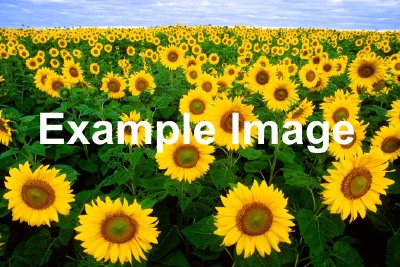
\includegraphics[width=0.5\textwidth]{images/Example.jpg}
		\caption{This is just an example image.}
		\label{fig:Example}
	\end{center}
\end{figure}

%This command prevents images from being floated too far away.
\FloatBarrier

\subsubsection{Adaptive Sampling}
\label{sec:Adaptive Sampling}

This is an example table taken from DIMA's IDB lecture slides:

\begin{table}[h!]
  \begin{tabular}{lccccccc}
	\toprule    
    \hline
    \textbf{Functions} & \multicolumn{3}{c}{\textbf{Framework}} && \multicolumn{2}{c}{\textbf{User Defined}}\\
    \cmidrule{2-4}  \cmidrule{6-7}  
    & Map & Shuffle & Reduce && Mapper &  Reducer\\
    \midrule
    \textbf{Input} & $ (K_m \times V_m)^{*} $ & $ (K_r \times V_r)^{*} $ & $ (K_r \times V_r^{*})^{*} $ && $ (K_m \times V_m) $  & $ (K_r \times V_r^{*}) $\\
    \hline
    \textbf{Output} & $ (K_r \times V_r)^{*} $ & $ (K_r \times V_r^{*})^{*} $ & $ (K_o \times V_o)^{*} $ && $ (K_r \times V_r)^{*} $ & $ (K_o \times V_o)^{*} $\\
	\hline    
    \bottomrule
  \end{tabular}
  \caption{Inputs and outputs of functions and processing phases in Map Reduce.}
  \label{table:mapRedFunctions}
\end{table}

And one more table:

\begin{table}[h!]
  \centering
  \begin{tabular}{lll}
	\toprule    
    \hline
    & \textbf{Input} & \textbf{Output}\\
    \midrule
    File Line 1:& Beer Beer Tea Coffee &\\
    File Line 2:& Tea Tea Beer Tea &\\
	\hline
	Map 1: & (1, Beer Beer Tea Coffee) & [(Beer,1),(Beer,1),(Tea,1),(Coffee,1)]\\
    Map 2: & (2, Tea Tea Beer Tea)     & [(Tea,1),(Tea,1),(Beer,1),(Tea,1)]\\
    \hline
    Reduce 1 & (Beer,[1,1,1])  & (Beer,3)\\  
	Reduce 2 & (Coffee,[1])    & (Coffee,1)\\
	Reduce 3 & (Tea,[1,1,1,1]) & (Tea,4)\\
    \hline    
    \bottomrule
  \end{tabular}
  \caption{Word Count Example: Sample data transformation.}
  \label{table:wcDataTransformation}
\end{table}

\subsubsection{Compressive Sampling}

You may want to use the description environment for your definitions.

Vocabulary introduced by Hirzel et al.~\cite{hirzel2014catalog} and inspired by Gamma et al.~\cite{gamma1995} and Fowler et al.~\cite{fowler1999}.

\begin{description}
	\item[Data Stream] \textit{A conceptual/possibly infinite sequence of data-items which comes from a stream source. Streaming systems implement streams as \ac{FIFO} queues.}
	\item[Stream Source] \textit{A stream source is a data source that possibly emits an infinite number of data-items.}
	\item[Operator] \textit{A code block , which consumes data-items from incoming stream(s) and produces data-items on outgoing stream(s). Thereby it performs a continuous data transformation.}
	\item[Query] \textit{A streaming query consists of operators which are vertices in a graph. The edges of the graph represent the data flow between operators. A streaming query combines multiple operations to a data transformation flow. Queries are also called \textit{applications}.}
	\item[Data-item] \textit{The smallest unit of data, which is processed by the streaming query, is called \emph{data-item}. It is also the smallest unit of communication along edges in the query. Anyhow, data-items can consist of several attributes.}
	\item[Window] \textit{A finite subsequence or chunk of data-items from a stream.}
\end{description}

\subsubsection{Data Sharing}
\label{sec:Listings}

Listing \ref{lst:SPLexample} is an example for a listing using lstlisting.

\begin{lstlisting}[float=b,label=lst:SPLexample,caption={An IBM SPL code example}]
stream<MyType> outputName = Aggregate(InputStream){
	window InputStream : sliding, delta(...), count(...);
	output outputName  : attribute1=Sum(a1*a2), attribute2=Sum(a3);
}
\end{lstlisting}

% Listings can also be imported from files like listing \ref{lst:samplecode}.
% \lstinputlisting[label=lst:samplecode,caption=A Java Hello World Program,language=java]{listings/helloWorld.java}
%Also use: firstline=300,lastline=500, linerange={10-17,20-35}


\subsection{Discussion}
\label{sec:Discussion}

Lorem ipsum dolor sit amet, consectetur adipisici elit, sed eiusmod tempor incidunt ut labore et dolore magna aliqua. Ut enim ad minim veniam, quis nostrud exercitation ullamco laboris nisi ut aliquid ex ea commodi consequat. Quis aute iure reprehenderit in voluptate velit esse cillum dolore eu fugiat nulla pariatur. Excepteur sint obcaecat cupiditat non proident, sunt in culpa qui officia deserunt mollit anim id est laborum.

\subsubsection{Other Algorithms}
\label{sec:Listings}

Lorem ipsum dolor sit amet, consectetur adipisici elit, sed eiusmod tempor incidunt ut labore et dolore magna aliqua. Ut enim ad minim veniam, quis nostrud exercitation ullamco laboris nisi ut aliquid ex ea commodi consequat. Quis aute iure reprehenderit in voluptate velit esse cillum dolore eu fugiat nulla pariatur. Excepteur sint obcaecat cupiditat non proident, sunt in culpa qui officia deserunt mollit anim id est laborum.


\subsubsection{Combination of Algorithms}
\label{sec:Listings}

Lorem ipsum dolor sit amet, consectetur adipisici elit, sed eiusmod tempor incidunt ut labore et dolore magna aliqua. Ut enim ad minim veniam, quis nostrud exercitation ullamco laboris nisi ut aliquid ex ea commodi consequat. Quis aute iure reprehenderit in voluptate velit esse cillum dolore eu fugiat nulla pariatur. Excepteur sint obcaecat cupiditat non proident, sunt in culpa qui officia deserunt mollit anim id est laborum.


\subsection{Acronyms}
\label{sec:Acronyms}

There are many acronyms provided in this template. You can use them as follows:
\begin{itemize}
	\item \acs{CSV} - The acs-command always uses the short form.
	\item \ac{CSV} - The ac-command uses the long form for the first appearance, then the short form.
	\item \acl{CSV} - The acl-command forces to use the long form.
	\item \acp{CSV} - When adding a 'p' to the mentioned commands, the plural form will be used.
\end{itemize}

\subsection{Citations}
You should read the publications from Albert Einstein~\cite{einstein1920relativity}.

\section{Conclusion}
\label{sec:Conclusion}

It is very important to have a good conclusion.

\clearpage
\mbox{}
\thispagestyle{empty}
\clearpage

%%%%%%%%%%% reference
\pagenumbering{roman}
\phantomsection
\addcontentsline{toc}{section}{References}
\bibliographystyle{plain}
\bibliography{bib}

%%%%%%%%%%% appendix

% \phantomsection
\addtocontents{toc}{\protect\newpage}
\addcontentsline{toc}{section}{Appendix}
\phantomsection
\section*{\begin{center}
Appendix
\end{center} }
\thispagestyle{empty}
\clearpage
\mbox{}
\thispagestyle{empty}
\clearpage
\pagenumbering{arabic}\renewcommand{\thepage}{A.\arabic{page}}
\appendix

\section{First entry in appendix}
\subsection{Subentry in appendix}
	\label{sec:Subentry in appendix}
	
Appendix is a Finnish punk rock band. It was founded in 1980 and has released five studio albums.
Their debut album was released in 1983. It was later re-issued by the German label Rock-O-Rama with an English title Money Is Not My Currency. Olli Lindholm, the lead singer of one of Finland's most selling rock groups Yö, is a former member of Appendix. (Source: Wikipedia)

\subsection{Another entry}

The appendix (or vermiform appendix; also cecal [or caecal] appendix; vermix; or vermiform process) is a blind-ended tube connected to the cecum, from which it develops embryologically. The cecum is a pouchlike structure of the colon, located at the junction of the small and the large intestines. The term "vermiform" comes from Latin and means "worm-shaped". (Source: Wikipedia) 

\end{document}
